\section{Grundlagen}

\subsection{Überblick}
Um unseren Lösungsansatz nachvollziehen zu können, ist es erforderlich, 
die Problemstellung detailliert zu analysieren. Im ersten Schritt wird betrachtet, 
welche Zielgruppe Ludwig System anspricht und welche spezifischen Optimierungen 
das Unternehmen verfolgt. Im Anschluss werden bestehende Lösungsansätze verglichen, 
um deren Stärken und Schwächen zu bewerten und als Grundlage 
für die Entwicklung eines verbesserten Systems zu nutzen.



\subsubsection{Anwendungsdomäne}
Das Abhängen von Lasten per Hand ist nicht nur zeitaufwendig, sondern oft auch gefährlich. 
Ludwig System bietet mit ihren funkgesteuerten Lasthaken eine innovative Lösung, 
die diese Arbeit deutlich erleichtert. Diese Haken ermöglichen es den Mitarbeitenden, 
Lasten aus sicherer Entfernung anzuheben und auszubalancieren. Besonders beliebt ist 
die Traverse, die speziell für den Transport von Dachelementen und Wänden entwickelt wurde. 
Allerdings müssen aktuelle Versionen noch manuell an die Last befestigt werden, 
was besonders bei hohen Wänden zeitaufwendig und gefährlich sein kann. 
Abbildung 2.2 illustriert die Nutzung der Traverse beim Transport eines Dachelements.


\begin{figure}[H]
    \centering
    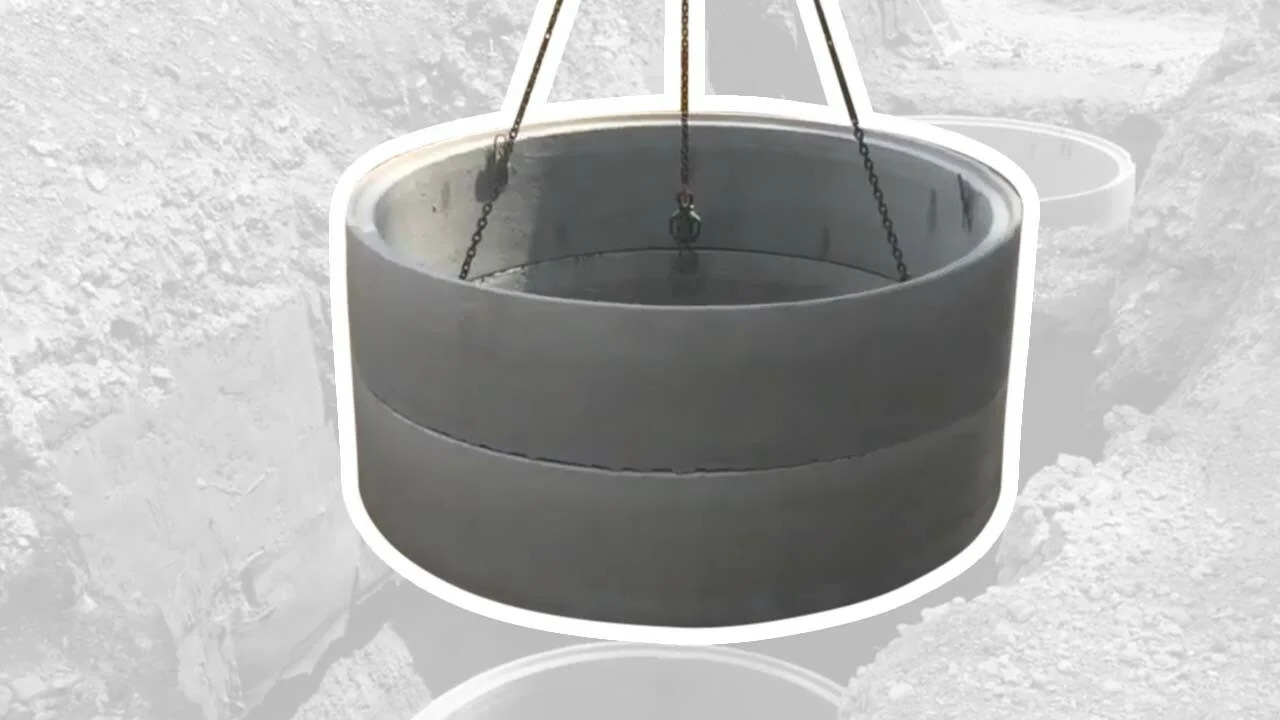
\includegraphics[width=0.5\textwidth]{graphics/Betonelement.jpg}\hfill%
    \caption{Ludwig Hook mit Betonelement}
    \centering
    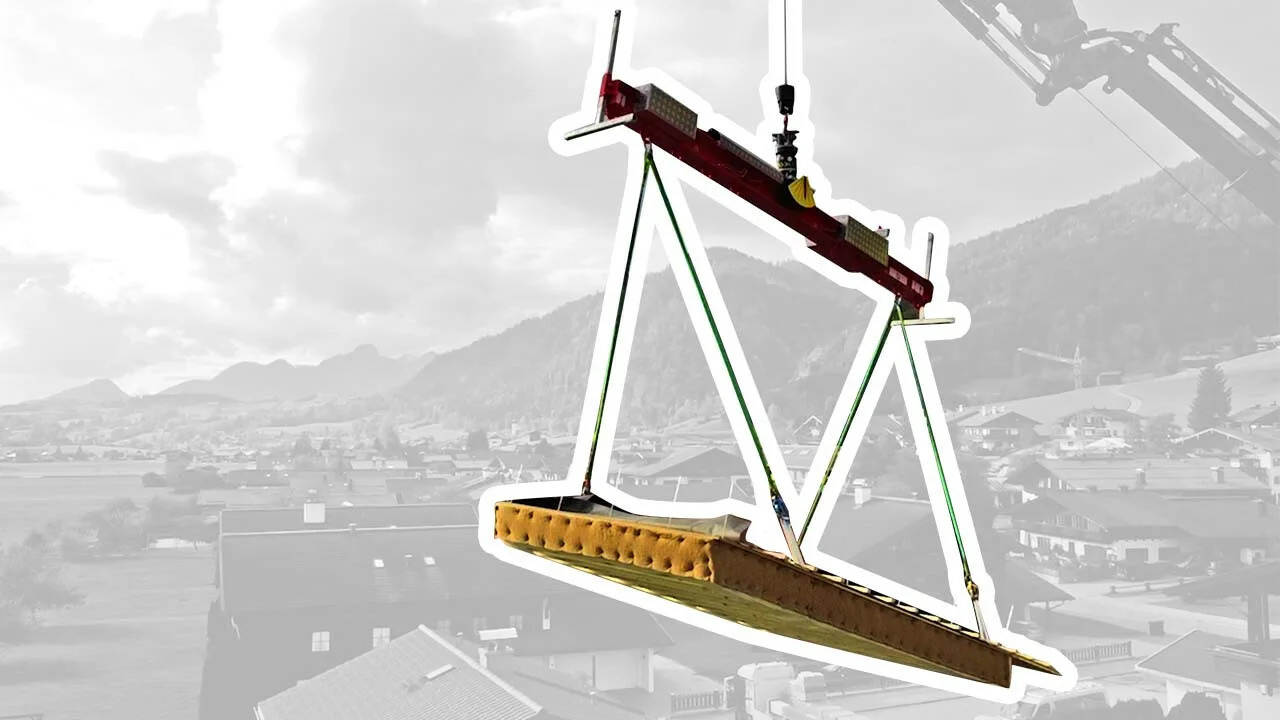
\includegraphics[width=0.5\textwidth]{graphics/Traverse.jpg}
    \caption{Traverse mit Dachelement}
\end{figure}

\subsubsection{Last}
Unter Lasten sind vor allem Fertigstrukturen wie z.B. Fertig erstellte Wände oder Dächer. Lasten haben maximal 2 Anschlagspunkte, welche einen Abstand von 1m bis 6m zueinander haben. Diese Anschlagspunkte können auf unterschiedliche Höchen sein, wie z.B. bei Dächer welche eine Neigung besitzen.


\clearpage
\subsubsection{Traverse}
Die LudwigTraverse ist eine Spezialtraverse, die speziell für den Lastausgleich entwickelt 
wurde. Sie erweist sich insbesondere dann als nützlich, wenn die Anschlagpunkte 
falsch positioniert sind und dadurch der Schwerpunkt der Last nicht korrekt berücksichtigt wird. 
Dies kann zu einer schrägen Ausrichtung beim Anheben der Last führen \cite{ludwigTraverse}.

\begin{figure}[H]
    \centering
    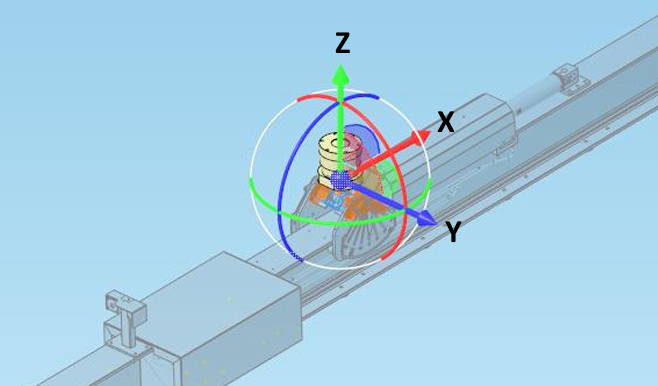
\includegraphics[width=0.5\linewidth]{graphics/Traverse_Rotationen.PNG}
    \caption{Koordinaten-System der Ludwig System Traverse}
    \label{fig:traverse}
\end{figure}

Abbildung \ref{fig:traverse} zeigt das linkshändige Koordinaten-System der Traverse.
Die Traverse hat Dimensionen (Länge × Breite y Höhe z) von 500 cm × 70 cm × 50 cm.
Dabei wird fortan die Rotation um die Y-Achse der Traverse als Neigen definiert und die Rotation 
um die Z-Achse der Traverse, als Rotieren definiert.


\subsection{Stand der Forschung}

\subsubsection{Arbeit: Objekterkennung und Distanzmessung für KollisionsVermeidung bei Lastenhebung}
(Arbeit: Object Detection and Distance Measurement Algorithm for Collision Avoidance of Precast Concrete Installation during Crane Lifting Process\cite{yong_object_2023} Erklären)

\subsubsection{Arbeit: Objekterkennung und 3D-basierte Objektortung für automatische Lastenhebung}
(Arbeit: Image-based onsite object recognition for automatic crane lifting tasks\cite{zhou_image-based_2021} Erklären)

\subsubsection{Arbeit: Erkennung von auf Robotersystemen angebrachten Passermarken}


\subsection{Passermarker}
Passermarker sind ein essenzielles Werkzeug in der modernen Bildverarbeitung und spielen eine 
zentrale Rolle in der räumlichen Orientierung und Positionsbestimmung. Insbesondere in Anwendungen 
wie der automatisierten Lastenhebung, wie sie von Ludwig System angestrebt wird, können Passermarker 
helfen, Anschlagpunkte präzise zu lokalisieren.

Diese Marker, darunter Barcodes, QR-Codes oder speziell entwickelte AR-Marker, liefern visuelle 
Referenzen, die von Kamerasystemen erkannt und interpretiert werden können. Damit ermöglichen sie es, 
Objekte im Raum genau zu positionieren oder auszurichten.

In diesem Abschnitt untersuchen wir die Grundlagen von Passermarkern und beleuchten ihre spezifischen 
Einsatzmöglichkeiten in unserem Szenario, insbesondere im Kontext der automatisierten Ausrichtung von 
Anschlagpunkten auf der Traverse.

\subsubsection{Einführung Passermarker}
Passermarker sind quadratische Muster, die auf flachen Oberflächen aufgedruckt werden. 
Sie dienen als visuelle Referenzpunkte, die von Kamerasystemen erkannt und interpretiert 
werden können. Es gibt verschiedene Arten von Passermarkern, die je nach Anwendung 
unterschiedliche Eigenschaften und Einsatzmöglichkeiten bieten. 
Abbildung \ref{fig:marker_types} zeigt eine Auswahl solcher Marker.

\begin{figure}[H]
    \centering
    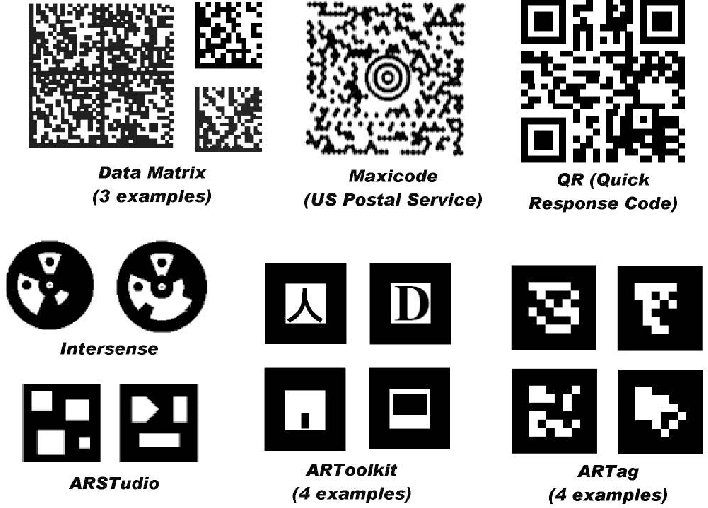
\includegraphics[width=0.5\linewidth]{graphics/marker_arten.png}
    \caption{Verschiedene Marker Arten}
    \label{fig:marker_types}
\end{figure}

Grundsätzlich gilt: Je komplexer und größer ein Marker ist, desto mehr Informationen können
darin gespeichert werden. Dabei muss jedoch der Informationsgehalt immer an die spezifischen 
Anforderungen der Anwendung angepasst werden, um eine optimale Balance zwischen Größe, Lesbarkeit 
und Informationsdichte zu gewährleisten.

In der Robotik gehören AprilTags und AruCo-Marker zu den meistgenutzten Passermarkern. 
Ihre Beliebtheit basiert auf ihrer Robustheit und Effizienz bei der Lokalisierung in 
dreidimensionalen Räumen. Diese Marker wurden speziell entwickelt, um Verzerrungen und 
schwierige Lichtverhältnisse zu kompensieren und eine präzise Posenschätzung zu ermöglichen. 
Ihre Anwendung wird im weiteren Verlauf dieser Arbeit genauer beleuchtet, insbesondere im 
Kontext der automatisierten Lokalisierung von Anschlagpunkten.


\subsubsection{Posenschätzung durch AR Marker}


\subsubsection{Probleme mit Passermarkern}



\subsection{Objekterkennung durch Machine Learning}
Künstliche Intelligenz (KI) spielt eine immer wichtigere Rolle in verschiedenen Bereichen 
unseres Lebens und wird auch in Zukunft zahlreiche Innovationen vorantreiben. 
Bereits heute revolutioniert sie viele Branchen, darunter die Automatisierung, 
Bildverarbeitung und Robotik. Eine besonders relevante Disziplin innerhalb der KI ist die 
Objekterkennung, die mithilfe von neuronalen Netzen umgesetzt wird.

Speziell für die vorliegende Problemstellung könnte eine KI entwickelt werden, die in der 
Lage ist, Anschlagpunkte unterschiedlicher Arten präzise zu erkennen und zu markieren. 
Durch den Einsatz von Machine-Learning-Modellen kann die Erkennung kontinuierlich verbessert 
werden, indem sie aus neuen Daten lernt und sich an verschiedene Szenarien und Bedingungen 
anpasst.

\subsubsection{Grundlagen Objekterkennung mit Neuronalen Netzen}
Neuronale Netzwerke sind inspiriert vom menschlichen Gehirn, bei dem Informationen zwischen Neuronen weitergegeben 
werden. Dabei verarbeitet jedes Neuron Signale und leitet sie verstärkt oder abgeschwächt an das nächste Neuron weiter.
Abbildung \ref{fig:humanCell} zeigt eine schematische Darstellung, wie Neuronen im menschlichen Gehirn miteinander 
kommunizieren.

\begin{figure}[H]
    \centering
    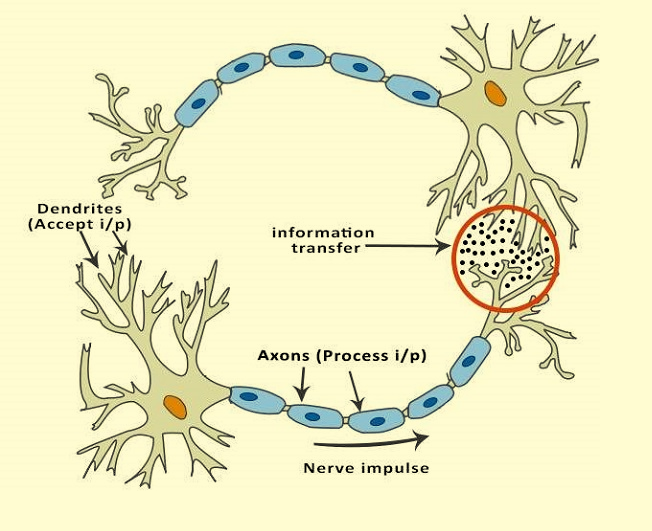
\includegraphics[width=0.5\linewidth]{graphics/human_model.png}
    \caption{Biologisches Neuron im menschlichen Gehirn}
    \label{fig:humanCell}
\end{figure}

Ähnlich wie das menschliche Gehirn Muster wie Kanten und Farben erkennen kann, werden künstliche neuronale Netzwerke 
darauf trainiert, Muster in numerischen Daten zu identifizieren. Maschinen sehen jedoch keine Bilder direkt, sondern 
verarbeiten Zahlenwerte (z. B. Pixelintensitäten), die aus den Bildern extrahiert werden. Dazu benötigen neuronale 
Netzwerke Parameter, die während des Trainingsprozesses optimiert werden. Zusätzlich wird ein Fehlersignal berechnet, 
wenn das Modell falsche Vorhersagen trifft, um das Lernen zu steuern.

Abbildung \ref{fig:network} zeigt die Struktur eines neuronalen Netzwerks mit drei Schichten: der Eingabeschicht (Input Layer), 
den verborgenen Schichten (Hidden Layers) und der Ausgabeschicht (Output Layer). Im Input Layer werden die Pixelwerte 
eines Bildes verarbeitet. Diese Werte werden mit den Gewichten der Verbindungen zwischen den Neuronen multipliziert, 
aufsummiert und an die nächste Schicht weitergegeben. In den Hidden Layers werden diese Berechnungen weitergeführt, 
bis im Output Layer eine Wahrscheinlichkeitsverteilung ausgegeben wird, die anzeigt, ob ein Anschlagspunkt im Bild 
vorhanden ist.

\begin{figure}[H]
    \centering
    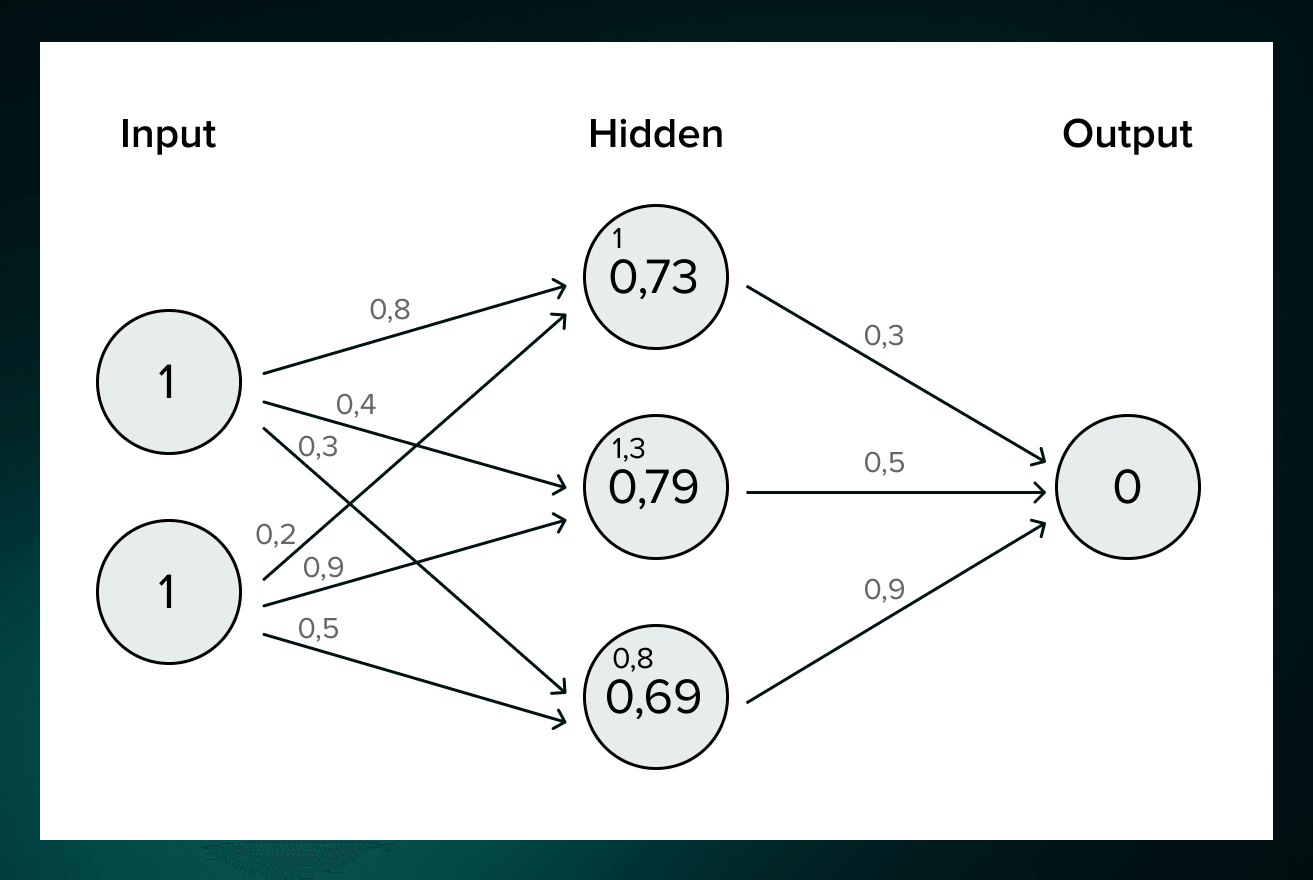
\includegraphics[width=0.5\linewidth]{graphics/network.png}
    \caption{Aufbau eines neuronalen Netzwerks}
    \label{fig:network}
\end{figure}

Damit ein Modell zuverlässig Anschlagspunkte erkennen kann, benötigt es Trainingsdaten, die korrekt klassifiziert sind. 
Während des Trainingsprozesses wird der Output des Modells mit den tatsächlichen Zielwerten verglichen, um den Verlust (Error) 
zu berechnen. Ziel ist es, diesen Verlust so gering wie möglich zu halten. Dies geschieht durch Optimierungsverfahren wie den 
Gradientenabstieg, bei dem die Ableitung der Verlustfunktion berechnet und zur Anpassung der Gewichte im Netzwerk verwendet wird.


\subsubsection{Vorhandene Modelle}


\subsubsection{Probleme mit Machine Learning}
Künstliche Intelligenz (KI) ist ein faszinierendes und vielversprechendes Thema, bringt 
jedoch einige Herausforderungen mit sich. Eines der Hauptprobleme ist der immense Bedarf 
an qualitativ hochwertigen Daten, die oft manuell aufbereitet und annotiert werden müssen. 
Dieser Prozess ist zeitaufwendig und erfordert erhebliche personelle und technische Ressourcen.

Darüber hinaus sind KI-Systeme in der Regel äußerst rechenintensiv. Wenn solche Systeme auf
einer Baustelle eingesetzt werden sollen, ist es oft notwendig, die Berechnungen remote in 
leistungsstarken Rechenzentren durchzuführen. Dies führt nicht nur zu zusätzlichen Kosten, 
sondern auch zu potenziellen Verzögerungen durch Latenzzeiten bei der Datenübertragung.

Ein weiteres Problem besteht darin, dass die KI allein anhand von Bilddaten ohne zusätzliche 
Informationen, wie etwa den genauen Dimensionen der Anschlagspunkte, Schwierigkeiten hat, 
präzise Berechnungen für die korrekte Ausrichtung der Traverse durchzuführen.
Dies verdeutlicht die Notwendigkeit einer Kombination aus KI-gestützter Objekterkennung und 
zusätzlichen sensorischen Daten, um zuverlässige Ergebnisse zu erzielen.

\subsection{Kameras}
\subsubsection{Kameraeigenschaften}
(Erklären was FOV, Verzerrrungen etc ist)
\subsubsection{Intrinsische Kalibrierung}
\subsubsection{Herausforderungen}

\subsection{Vorhandene Frameworks}
(Erklärung von OpenCV und ihren Methoden)

